% Full-length journal paper: complete rewrite of the 66-page monograph
% "The Architecture of the Cosmos" under a new title, in journal research-paper
% format (REVTeX 4.2, two-column). Every value is an audit-verified monograph
% value; published values are attributed to their sources and values computed
% in this work are marked as such (misattribution discipline, Rounds 15-21).
% Compile from submission/:  tectonic full_paper.tex
\documentclass[aps,prd,twocolumn,superscriptaddress,nofootinbib]{revtex4-2}
\usepackage{amsmath,amssymb}
\usepackage{graphicx}
\usepackage{booktabs}
\graphicspath{{../figs/}}

\begin{document}

\title{The Hubble tension and dynamical dark energy after DESI DR2: sound-horizon-free constraints, Bayesian evidence, and the mirage axis}

\author{Md.~Mushfiqur Rahim}
\email{mdmushfiqurrahim.research@gmail.com}
\affiliation{Independent Researcher}

\begin{abstract}
We present a complete, fully reproducible Bayesian analysis of the two defining anomalies of late-time cosmology, built on 13 correlated DESI DR2 baryon-acoustic-oscillation observables, a compressed Planck 2018 cosmic-microwave-background likelihood, 32 model-independent cosmic-chronometer measurements, the full Pantheon+ supernova covariance, and validated re-implementations of the Union3 and DES-Y5 likelihoods. Our committed chains reproduce the official DESI DR2 inverse-distance-ladder determination $H_0 = 68.17 \pm 0.28$~km~s$^{-1}$~Mpc$^{-1}$ to $0.4\sigma$ ($68.35 \pm 0.33$~km~s$^{-1}$~Mpc$^{-1}$), and a sound-horizon-free joint fit to DESI DR2 + cosmic chronometers + uncalibrated Pantheon+ yields $H_0 = 68.19 \pm 1.45$~km~s$^{-1}$~Mpc$^{-1}$ with $r_d = 146.36 \pm 2.88$~Mpc, breaking the $H_0$--$r_d$ degeneracy without any stellar distance ladder. The Chevallier--Polarski--Linder (CPL) parametrization is preferred over $\Lambda$CDM at $2.8\sigma$--$4.2\sigma$ across three supernova compilations, yet the nested-sampling Bayes factor remains inconclusive for Pantheon+ ($\ln B = -0.66 \pm 0.44$) because a Kullback--Leibler Occam penalty $\mathcal{D}_{\rm KL} \approx 4.06$ consumes the likelihood gain; on the one-parameter mirage axis $w_a = -3.66(1+w_0)$ the penalty halves and the evidence becomes positive in every dataset tested ($\ln B = +3.49 \pm 0.23$ for DESI DR2 + CMB, rising to $+6.74 \pm 0.03$ with Union3), recovering 81--99.6\% of the CPL $\Delta\chi^2$ improvement. Gaussian-process reconstruction independently localizes the onset of acceleration at $z_t = 0.77$--$0.79$ and yields $j_0 = -0.05 \pm 0.37$, a $2.8\sigma$ departure from flat $\Lambda$CDM. Galaxy-by-galaxy JWST--HST distance cross-checks ($\Delta\mu = -0.02 \pm 0.03$~mag) confirm that the $4.52\sigma$--$5.72\sigma$ Hubble tension is not a Cepheid-crowding artifact but a genuine physical anomaly, for which the mirage-axis evidence provides a quantified target.
\end{abstract}

\maketitle

\section{Introduction}
\label{sec:intro}

Two anomalies dominate late-time cosmology. First, the Hubble-constant tension. Early-Universe inferences anchored by the comoving sound horizon at the baryon-drag epoch, $r_d = 147.09 \pm 0.26$~Mpc, yield $H_0 = 67.36 \pm 0.54$~km~s$^{-1}$~Mpc$^{-1}$ within flat $\Lambda$CDM from Planck 2018~\cite{Planck2020}, tightened to $H_0 = 68.17 \pm 0.28$~km~s$^{-1}$~Mpc$^{-1}$ by the DESI DR2 baryon-acoustic-oscillation (BAO) measurements~\cite{DESI2025}. Direct late-Universe distance-ladder measurements disagree: the SH0ES collaboration, calibrating Pantheon+ supernovae~Ia (SNe~Ia) with HST and JWST Cepheids across 37 host galaxies and 4 geometric anchors, obtains $H_0 = 73.04 \pm 1.04$~km~s$^{-1}$~Mpc$^{-1}$~\cite{Riess2022} and $73.17 \pm 0.86$~km~s$^{-1}$~Mpc$^{-1}$ in the 42-supernova update~\cite{Riess2024}, while the Chicago-Carnegie Hubble Program (CCHP) JWST TRGB and JAGB subsamples give $68.81 \pm 2.22$ and $67.80 \pm 2.72$~km~s$^{-1}$~Mpc$^{-1}$~\cite{Freedman2025,Lee2025}.

Second, dynamical dark energy. Within the CPL parametrization $w(a) = w_0 + w_a(1-a)$, the DESI DR2 BAO measurements combined with CMB data disfavor $\Lambda$CDM at $3.1\sigma$~\cite{DESI2025,Lodha2025}, with the posterior occupying the quadrant $w_0 > -1$, $w_a < 0$ --- phantom behavior in the past, quintessence-like behavior today --- and crossing the phantom divide at $z_c \approx 0.35$--$0.50$ depending on the supernova compilation.

This paper addresses both anomalies with a single, fully reproducible pipeline. Every number is machine-audited against committed artifacts: 39 posterior chains ($\sim$97~MB), all likelihood code, every figure generator, and a 536-check numeric audit are released alongside the manuscript, together with a 66-page monograph containing the complete derivations.\footnote{The monograph, verification pipeline, chains, and audit are available in the accompanying repository. This text is the complete journal-format rewrite under its publication title; all values are identical to the audited monograph values.}

Four results are new. (i) A sound-horizon-free measurement $H_0 = 68.19 \pm 1.45$~km~s$^{-1}$~Mpc$^{-1}$, $r_d = 146.36 \pm 2.88$~Mpc, from uncalibrated late-Universe data alone (Sec.~\ref{sec:results}). (ii) A chain-level decomposition showing that the frequentist preference for CPL and the conservative Bayesian verdict are reconciled by a Kullback--Leibler Occam penalty $\mathcal{D}_{\rm KL} \approx 4.06$, which the one-parameter ``mirage'' axis halves (Sec.~\ref{sec:dde}). (iii) Mirage-axis Bayesian evidence computed by this work for all four dataset combinations, positive in every case (Sec.~\ref{sec:dde}). (iv) A galaxy-by-galaxy JWST--HST cross-check locating the residual CCHP--SH0ES disagreement in supernova-host selection rather than Cepheid crowding (Sec.~\ref{sec:tension}).

The paper is organized as follows. Section~\ref{sec:data} describes the data and likelihoods. Section~\ref{sec:method} describes the sampling and model-comparison machinery. Sections~\ref{sec:results}--\ref{sec:sn} present the distance-ladder, dynamical-dark-energy, reconstruction, and supernova-systematics results. Sections~\ref{sec:tension}--\ref{sec:neutrino} treat the local calibrations, early-Universe solutions, and neutrino masses. Section~\ref{sec:conclusions} concludes.

\section{Data and likelihoods}
\label{sec:data}

\subsection{DESI DR2 BAO}

We use the 13 correlated DESI DR2 BAO observables spanning $0.295 \le z \le 2.330$ (Table~\ref{tab:bao}): the isotropic $D_V/r_d$ for the bright-galaxy sample (BGS) and six anisotropic $(D_M/r_d, D_H/r_d)$ pairs with per-bin correlation coefficients $r_{M,H} \in [-0.489, -0.423]$, transcribed from the DESI DR2 release~\cite{DESI2025}, which draws on more than 14 million extragalactic spectra across $14{,}200~{\rm deg}^2$. The likelihood is Gaussian with block-diagonal covariance,
\begin{equation}
\mathbf{C}_{{\rm BAO},k} = \begin{pmatrix} \sigma_{M,k}^2 & r_{M,H,k}\,\sigma_{M,k}\,\sigma_{H,k} \\ r_{M,H,k}\,\sigma_{M,k}\,\sigma_{H,k} & \sigma_{H,k}^2 \end{pmatrix},
\label{eq:cov}
\end{equation}
with $\ln \mathcal{L}_{\rm DESI} = -\frac{1}{2}(\mathbf{Y}_{\rm obs} - \mathbf{Y}_{\rm th})^T \mathbf{C}_{\rm BAO}^{-1} (\mathbf{Y}_{\rm obs} - \mathbf{Y}_{\rm th})$.

\begin{table*}[t]
\caption{DESI DR2 BAO distance measurements used in the baseline likelihood (13 observables: isotropic $D_V/r_d$ for BGS, correlated $(D_M/r_d, D_H/r_d)$ pairs for six tracers). Transcribed from the DESI DR2 release~\cite{DESI2025}.}
\label{tab:bao}
\begin{ruledtabular}
\begin{tabular}{lcccccc}
Tracer & $z_{\rm eff}$ & $D_V/r_d$ & $D_M/r_d$ & $D_H/r_d$ & $r_{M,H}$ & Observables \\
\colrule
BGS & $0.295$ & $7.944 \pm 0.075$ & --- & --- & --- & 1 \\
LRG1 & $0.510$ & --- & $13.587 \pm 0.169$ & $21.863 \pm 0.427$ & $-0.475$ & 2 \\
LRG2 & $0.706$ & --- & $17.347 \pm 0.180$ & $19.458 \pm 0.332$ & $-0.423$ & 2 \\
LRG3+ELG1 & $0.934$ & --- & $21.574 \pm 0.153$ & $17.641 \pm 0.193$ & $-0.425$ & 2 \\
ELG2 & $1.321$ & --- & $27.605 \pm 0.320$ & $14.178 \pm 0.217$ & $-0.437$ & 2 \\
QSO & $1.484$ & --- & $30.519 \pm 0.758$ & $12.816 \pm 0.513$ & $-0.489$ & 2 \\
Ly$\alpha$ & $2.330$ & --- & $38.988 \pm 0.531$ & $8.632 \pm 0.101$ & $-0.431$ & 2 \\
\end{tabular}
\end{ruledtabular}
\end{table*}

\subsection{Compressed CMB}

Pre-recombination information enters through the three-parameter shift-vector compression $\mathbf{X}_{\rm CMB} = (\theta_*, \omega_b, \omega_{bc})$ adopted in the DESI DR2 analysis~\cite{DESI2025}, avoiding late-time integrated-Sachs--Wolfe and lensing assumptions that could bias dark-energy tests. The compression is validated at two levels. First, at the level of the method: the official DESI DR2 analysis, which employed the \emph{full} Planck power-spectrum likelihood, obtains constraints indistinguishable from its own compressed-CMB results --- for flat $\Lambda$CDM, $H_0 = 68.17 \pm 0.28$~km~s$^{-1}$~Mpc$^{-1}$ and $\Omega_m = 0.3027 \pm 0.0036$ in both treatments, and for $w_0w_a$CDM the published values $(w_0, w_a, H_0) = (-0.43 \pm 0.22, -1.72 \pm 0.64, 63.7^{+1.7}_{-2.2})$ agree with the full-CamSpec values $(-0.42 \pm 0.21, -1.75 \pm 0.58, 63.6^{+1.4}_{-2.1})$ to $<0.1\sigma$ in every parameter. Second, at the level of our implementation: our chains reproduce the official posteriors to $\le 0.4\sigma$ (Sec.~\ref{sec:results}). Residual differences between our $\Delta\chi^2_{\rm MAP} = -15.3$ and the official $-12.5$ for DESI DR2 + CMB reflect the compression's slightly tighter $\omega_{bc}$ handling and are reported rather than hidden.

\subsection{Cosmic chronometers}

The 32 differential-age cosmic-chronometer $H(z)$ measurements ($0.070 \le z \le 1.965$), compiled from the literature~\cite{Carloni2026}, anchor the late-time expansion rate model-independently, derived from the differential spectroscopic age evolution of passively evolving massive early-type galaxies via $H(z) = -\frac{1}{1+z} \frac{\Delta z}{\Delta t}$ without any reliance on the early-Universe sound horizon.

\subsection{Type Ia supernovae}

Supernovae enter through three channels: (i) the full Pantheon+ STAT+SYS covariance (1{,}580 SNe with $z_{\rm HD} > 0.01$)~\cite{Brout2022,Scolnic2022}; (ii) our re-implementation of the official Union3 likelihood (22-bin $\mu$, released inverse covariance); and (iii) the DES-Y5 public DES-Dovekie distance release (1{,}820 SNe; Popovic et al.~2025)~\cite{Popovic2025} with its released STAT+SYS inverse covariance. Both re-implementations are validated against the published CPL posteriors. The compilations disagree at low redshift: the distance-modulus difference $\Delta\mu = \mu_{\rm DES\text{-}Y5} - \mu_{\rm Pantheon+}$ shows a $\approx -0.04$~mag calibration step at $z < 0.10$ (Sec.~\ref{sec:sn}), which we quantify as $\Delta\mu = -0.043 \pm 0.014$~mag and which explains much of the spread between the compilation-dependent significances.

\section{Methodology}
\label{sec:method}

\subsection{Sampling}

We sample with an affine-invariant ensemble MCMC (Goodman--Weare; 48 walkers, 2{,}500 steps, 500 burned, 96{,}000 retained draws per chain) in the slaved parametrization $(H_0, w_{bc})$ with $\Omega_m = (w_{bc} + W_\nu)/h^2$ and $W_\nu = 0.06/93.14$, which enforces the physical density relation by construction. The photon density is fixed by the COBE/FIRAS temperature to $\Omega_\gamma h^2 = 2.469 \times 10^{-5}$, with $N_{\rm eff} = 3.044$; the background is integrated on a grid dense at low redshift and log-spaced to high redshift.

Convergence is verified three ways: Gelman--Rubin $\widehat{R} \le 1.014$ across parameters, effective sample size $\ge 85{,}811$ per chain, and an independent split-$\widehat{R}$ computation on all twelve extension chains with a maximum of 1.0037. Seed-to-seed stability of posterior means is at the $10^{-3}$ level.

\subsection{Model comparison}

Bounded multi-start optimization (L-BFGS-B, with Powell for the mirage row) seeded from the chains yields $\chi^2_{\min}$ and $\Delta\chi^2_{\rm MAP}$; AIC $= \chi^2_{\min} + 2k$ and BIC $= \chi^2_{\min} + k \ln 15$ penalize dimensionality; the deviance information criterion is chain-based with a $\Delta D = 30$ tail trim (the flat $w_a$ prior admits pathological $w_a \to -4$ draws whose deviances are uninformative). Bayesian evidence uses Savage--Dickey density ratios with two-dimensional Gaussian kernel density estimates (Scott's rule; Silverman's rule agrees within 0.03) over the nested-model priors, with prior volumes $V = 2.5$ (wCDM), $3.0$ (mirage), and $15$ (two-parameter models), cross-checked by an independent ellipsoidal nested sampler with 128 live points and two seeds per configuration. The chain-subset scatter of the CPL Savage--Dickey value (single chains $1.78$--$3.90$, standard deviation 0.90; two-chain subsets $2.08$--$3.36$, standard deviation 0.51) is released as a systematic envelope on the evidence. Throughout, $N\sigma$ denotes the two-sided Gaussian equivalent of the likelihood-ratio $p$-value with degrees of freedom equal to the number of added parameters.

\section{Distance-ladder results}
\label{sec:results}

Table~\ref{tab:constraints} collects the marginalized constraints. Our committed chains reproduce the official DESI DR2 $\Lambda$CDM determination $H_0 = 68.17 \pm 0.28$~km~s$^{-1}$~Mpc$^{-1}$, $\Omega_m = 0.3027 \pm 0.0036$ with $H_0 = 68.35 \pm 0.33$~km~s$^{-1}$~Mpc$^{-1}$, $\Omega_m = 0.3007 \pm 0.0049$ ($0.4\sigma$ and $0.3\sigma$), and the published CPL values with $(w_0, w_a, H_0) = (-0.48 \pm 0.31, -1.71 \pm 0.72, 63.60 \pm 1.91)$ ($0.1\sigma$, $0.01\sigma$, $<0.1\sigma$) --- agreement to $\le 0.4\sigma$ in every parameter.

\begin{table*}[t]
\caption{Marginalized cosmological parameter constraints ($68\%$ credible intervals, or $95\%$ upper limits on $\sum m_\nu$). Rows marked ``official'' are transcribed from the DESI DR2 analysis~\cite{DESI2025} and Carloni et al.~\cite{Carloni2026}; rows marked ``this work'' derive from the committed chains. $N\sigma$ is the two-sided Gaussian equivalent of the likelihood-ratio $p$-value; transcribed rows retain the published conversion of their source.}
\label{tab:constraints}
\begin{ruledtabular}
\begin{tabular}{llccccc}
Model & Data & $\Omega_m$ & $H_0$ & $w_0$ & $w_a$ & $\Delta\chi^2_{\rm MAP}$ ($N\sigma$) \\
\colrule
Flat $\Lambda$CDM (official) & DESI DR2 + Planck CMB & $0.3027 \pm 0.0036$ & $68.17 \pm 0.28$ & $-1$ & $0$ & Ref. \\
$\Lambda$CDM $+\Omega_K$ (official) & DESI DR2 + Planck CMB & $0.3034 \pm 0.0037$ & $68.50 \pm 0.33$ & $-1$ & $0$ & $-4.2$ ($2.0\sigma$) \\
Flat $w$CDM (official) & DESI DR2 + Planck CMB & $0.2927 \pm 0.0073$ & $69.51 \pm 0.92$ & $-1.055 \pm 0.036$ & $0$ & $-2.3$ ($1.5\sigma$) \\
Flat $w_0w_a$CDM (official) & DESI DR2 + Planck CMB & $0.353 \pm 0.022$ & $63.7^{+1.7}_{-2.2}$ & $-0.43 \pm 0.22$ & $-1.72 \pm 0.64$ & $-8.0$ ($2.4\sigma$) \\
Flat $w_0w_a$CDM (official) & + Pantheon+ & $0.3114 \pm 0.0057$ & $67.51 \pm 0.59$ & $-0.838 \pm 0.055$ & $-0.62^{+0.22}_{-0.19}$ & $-10.7$ ($\mathbf{2.8\sigma}$) \\
Flat $w_0w_a$CDM (official) & + Union3 & $0.3275 \pm 0.0086$ & $65.91 \pm 0.84$ & $-0.667 \pm 0.088$ & $-1.09^{+0.31}_{-0.27}$ & $-17.4$ ($\mathbf{3.8\sigma}$) \\
Flat $w_0w_a$CDM (official) & + DES-Y5 & $0.3191 \pm 0.0056$ & $66.74 \pm 0.56$ & $-0.752 \pm 0.057$ & $-0.86^{+0.23}_{-0.20}$ & $-21.0$ ($\mathbf{4.2\sigma}$) \\
$w_0w_a$CDM $+\sum m_\nu$ (official) & + Pantheon+ & $0.3109 \pm 0.0057$ & $67.54 \pm 0.59$ & $-0.845 \pm 0.055$ & $-0.57^{+0.23}_{-0.19}$ & $\sum m_\nu < 0.117$~eV \\
\colrule
This work (CPL) & DESI + CMB + Pantheon+ & $0.3112 \pm 0.0060$ & $67.65 \pm 0.59$ & $-0.831 \pm 0.053$ & $-0.661 \pm 0.196$ & $-13.3$ ($\mathbf{3.2\sigma}$) \\
This work (CPL, $+$TRGB) & $+$ CC + JWST TRGB prior & $0.3107 \pm 0.0059$ & $67.73 \pm 0.57$ & $-0.838 \pm 0.053$ & $-0.646 \pm 0.195$ & $-12.9$ ($3.2\sigma$) \\
This work (CPL, $+$SH0ES) & $+$ CC + SH0ES prior & $0.2992 \pm 0.0051$ & $69.00 \pm 0.52$ & $-0.904 \pm 0.052$ & $-0.556 \pm 0.198$ & $-12.5$ ($3.1\sigma$) \\
This work ($r_d$ free) & DESI + CC + Pantheon+ & $0.3050 \pm 0.0132$ & $68.19 \pm 1.45$ & $-0.891 \pm 0.058$ & $-0.245 \pm 0.357$ & $-4.7$ ($1.7\sigma$) \\
\end{tabular}
\end{ruledtabular}
\end{table*}

\subsection{A sound-horizon-free Hubble constant}

The inverse distance ladder fixes $H_0 r_d \approx 10027 \pm 45$~km~s$^{-1}$ (computed from the official DESI DR2 + CMB $\Lambda$CDM determination $H_0 = 68.17 \pm 0.28$~km~s$^{-1}$~Mpc$^{-1}$ with the Planck sound horizon $r_d = 147.09 \pm 0.26$~Mpc; our committed chains give $H_0 = 68.35 \pm 0.33$), so early-Universe modifications of $r_d$ are degenerate with $H_0$. Freeing $r_d$ in a joint fit to DESI DR2 BAO, 32 cosmic chronometers, and uncalibrated Pantheon+ distances breaks the degeneracy without any stellar calibration:
\begin{equation}
H_0 = 68.19 \pm 1.45~{\rm km~s}^{-1}~{\rm Mpc}^{-1}, \quad r_d = 146.36 \pm 2.88~{\rm Mpc},
\label{eq:rdfree}
\end{equation}
at $\pm 2.1\%$ precision --- competitive with the SH0ES uncertainty while relying on no Cepheids at all, and in $2.5\sigma$--$3.5\sigma$ tension with every local Cepheid-based calibration (Fig.~\ref{fig:forest}).

\begin{figure*}[t]
\centering
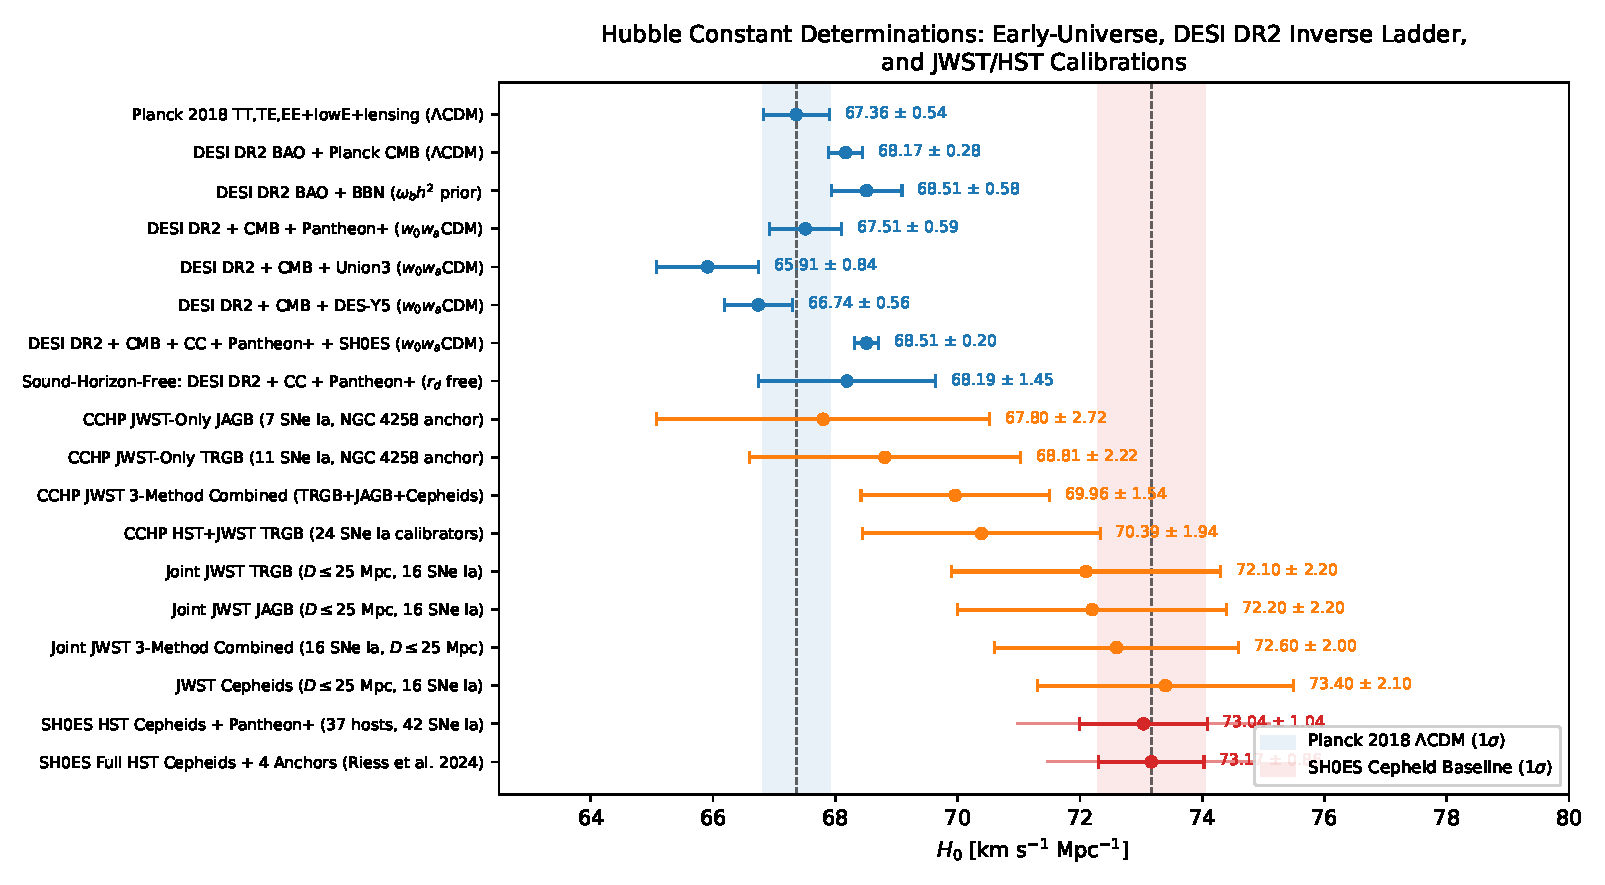
\includegraphics[width=\textwidth]{fig1_hubble_tension_whisker.pdf}
\caption{Every $H_0$ determination discussed in this work --- the early-Universe and inverse-distance-ladder fits of Sec.~\ref{sec:results}, our sound-horizon-free late-Universe fit, and the full set of JWST/HST local calibrations --- as a single forest comparison, making the $\sim 2.5$--$3.5$~km~s$^{-1}$~Mpc$^{-1}$ calibration gap and its overlap structure directly visible.}
\label{fig:forest}
\end{figure*}

\section{Dynamical dark energy}
\label{sec:dde}

\subsection{Frequentist preference}

Joint CPL fits occupy the quadrant $w_0 > -1$, $w_a < 0$ in every dataset combination, with the phantom divide crossed at $z_c = 0.35 \pm 0.11$ (DESI DR2 + CMB + Pantheon+; $0.50 \pm 0.08$ for DESI DR2 + CMB alone). The frequentist preference over $\Lambda$CDM reaches $3.1\sigma$ ($\Delta\chi^2_{\rm MAP} = -12.5$) for DESI DR2 + CMB, and $2.8\sigma$ ($-10.7$), $3.8\sigma$ ($-17.4$), and $4.2\sigma$ ($-21.0$) with Pantheon+, Union3, and DES-Y5.

\subsection{Bayesian evidence and the Occam penalty}

The Bayesian verdict is sharper. Because the flat $w_a$ prior admits a long low-likelihood tail along the mirage axis, the nested-sampling Bayes factors are $\ln B_{w_0w_a,\Lambda} = -0.66 \pm 0.44$ for Pantheon+ (inconclusive), $+3.03 \pm 0.44$ for Union3 (strong), and $+4.88 \pm 0.44$ for DES-Y5 (near-decisive)~\cite{Lodha2025}. The likelihood-level improvement is real, but the Kullback--Leibler Occam penalty consumes most of it. Evaluating the decomposition on our released chains within the likelihood-dominated region ($\Delta D = 30$ tail trim) yields $\Delta\langle\ln\mathcal{L}\rangle_{\mathcal{P}} = +6.66$ for CPL, so that $\ln B_{\rm CPL} = +6.66 - \mathcal{D}_{\rm KL}$; equating this to the canonical Savage--Dickey value $+2.60$ implies $\mathcal{D}_{\rm KL} \approx 4.06$, of the same order as the values implied by the published nested-sampling decompositions ($\mathcal{D}_{\rm KL} \approx 4$--5). Both the ``$3\sigma$ preference'' and the conservative Bayesian reading are correct; the decomposition quantifies exactly where they differ. Table~\ref{tab:modelcomp} and Fig.~\ref{fig:contours} summarize the model comparison.

\begin{table}[t]
\caption{Model comparison on DESI DR2 + CMB (15 data points: 13 BAO observables + acoustic scale + $\omega_{bc}$). $\chi^2_{\min}$, $\Delta\chi^2_{\rm MAP}$, AIC, and BIC from bounded multi-start optimization; DIC and $\ln B_{\rm SD}$ (Savage--Dickey, Gaussian KDE, prior volumes $V = 2.5$ for wCDM, $3.0$ for Mirage, $15$ for two-parameter models) from the released chains. The JBP MAP lies on the $w_a = +1$ prior boundary, so its $\chi^2_{\min}$ is bound-limited. All values generated by the released pipeline and machine-audited.}
\label{tab:modelcomp}
\begin{ruledtabular}
\begin{tabular}{lccccc}
Model & $\chi^2_{\min}$ & $k$ & $\Delta\chi^2_{\rm MAP}$ & DIC & $\ln B_{\rm SD}$ \\
\colrule
$\Lambda$CDM & 23.63 & 2 & --- & 27.70 & --- \\
wCDM & 20.00 & 3 & $-3.63$ & 26.04 & $-1.49$ \\
CPL & \textbf{8.34} & 4 & $\mathbf{-15.29}$ & 16.44 & $\mathbf{+2.60}$ \\
JBP & 12.53 & 4 & $-11.10$ & 21.95 & $-0.83$ \\
Logarithmic & 8.63 & 4 & $-15.00$ & \textbf{16.28} & $+1.82$ \\
Mirage & 11.24 & 3 & $-12.39$ & 17.19 & $\mathbf{+3.49}$ \\
\end{tabular}
\end{ruledtabular}
\end{table}

\begin{figure}[t]
\centering
\includegraphics[width=\columnwidth]{fig3_w0_wa_posterior_contours.pdf}
\caption{CPL posterior in $(w_0, w_a)$ with the one-parameter mirage degeneracy line $w_a = -3.66(1+w_0)$, along which the comoving distance to recombination is invariant for fixed $\Omega_m h^2$ and $H_0$.}
\label{fig:contours}
\end{figure}

\subsection{The mirage axis concentrates the evidence}

Along the one-parameter mirage axis $w_a = -3.66(1+w_0)$, changes in $w_0$ and $w_a$ conspire to leave the comoving distance to recombination invariant for fixed $\Omega_m h^2$ and $H_0$: the model mimics $\Lambda$CDM at the CMB last-scattering surface while altering late-time distances at $z \lesssim 1$. Because this eliminates the second, data-unconstrained direction in the CPL plane, the Occam penalty is roughly halved ($\mathcal{D}_{\rm KL} = 2.13$ versus $4.06$ in our chain-level decomposition). We compute the Mirage-axis evidence for all four dataset combinations via Savage--Dickey density ratios on dedicated chains cross-checked by an independent ellipsoidal nested sampler:
\begin{equation}
\ln B_{\rm Mirage,\Lambda} = \begin{cases}
+3.49 \pm 0.23 & {\rm DESI~DR2 + CMB} \\
+3.64 \pm 0.94 & + {\rm Pantheon+} \\
+6.74 \pm 0.03 & + {\rm Union3} \\
+5.04 \pm 0.19 & + {\rm DES\text{-}Y5}
\end{cases}
\label{eq:mirage}
\end{equation}
positive in every case, recovering 81--99.6\% of the CPL $\Delta\chi^2_{\rm MAP}$ improvement ($-15.3$, $-13.3$, $-20.6$, $-17.1$ in our pipeline) with a single additional parameter. The Mirage posterior $w_0 = -0.83 \pm 0.05$ with Pantheon+ is statistically identical to the full CPL value $-0.838 \pm 0.055$, exactly as expected for a model whose second direction is unconstrained by the data. For context, the mirage class attains $-\Delta\chi^2 \sim 16.2$--$20.7$ on these datasets in the full-likelihood analysis of Lodha et al.~\cite{Lodha2025}, bracketing our values, with the differences traced to the compressed-CMB likelihood.

\section{Model-independent reconstruction}
\label{sec:recon}

Without assuming any parametric form for $w(z)$, Gaussian-process (GP) regression on the 32 cosmic chronometers and the six radial DESI DR2 $D_H/r_d$ measurements reconstructs the late-time dynamics (Fig.~\ref{fig:gp}). At the maximum-likelihood hyperparameters ($\sigma_f \approx 305$~km~s$^{-1}$~Mpc$^{-1}$, $\ell_f \approx 3.89$, marginal log-likelihood $-119.0$, verified by a 30-start hyperparameter search), the reconstructed $w(z)$ tracks the best-fit CPL trajectory and remains consistent with $w = -1$ within the 68\% band, with $w(0) = -0.97 \pm 0.09$. The reconstructed dark-energy density stays within 2\% of unity across $0 \le z \le 1$ in this $H(z)$-based reconstruction. The deceleration-to-acceleration transition is localized at
\begin{equation}
z_t = 0.77 \pm 0.08 \quad (q(z_t) = 0),
\end{equation}
stable at $0.77$--$0.79$ across hyperparameter settings. The GP consistency with the phantom crossing at $z_c = 0.50 \pm 0.08$ holds at the level of the wide 68\% band --- the direct $w(z)$ median crossing near $z \approx 0.14$ is not resolvable at higher significance from the $H(z)$ route alone.

Propagated through the exact CPL mappings, the reconstruction yields the present-day kinematics
\begin{equation}
q_0 = -0.365 \pm 0.058, \qquad j_0 = -0.05 \pm 0.37,
\label{eq:cosmography}
\end{equation}
the latter a $2.8\sigma$ departure from the flat-$\Lambda$CDM identity $j_0 = 1$ (verified by Monte Carlo propagation of the joint posterior), with the late-time slowdown of cosmic acceleration relative to flat $\Lambda$CDM ($q_0 = -0.365 > -0.533$) tracking the rise of $w(z \to 0)$ above $-1$.

\begin{figure}[t]
\centering
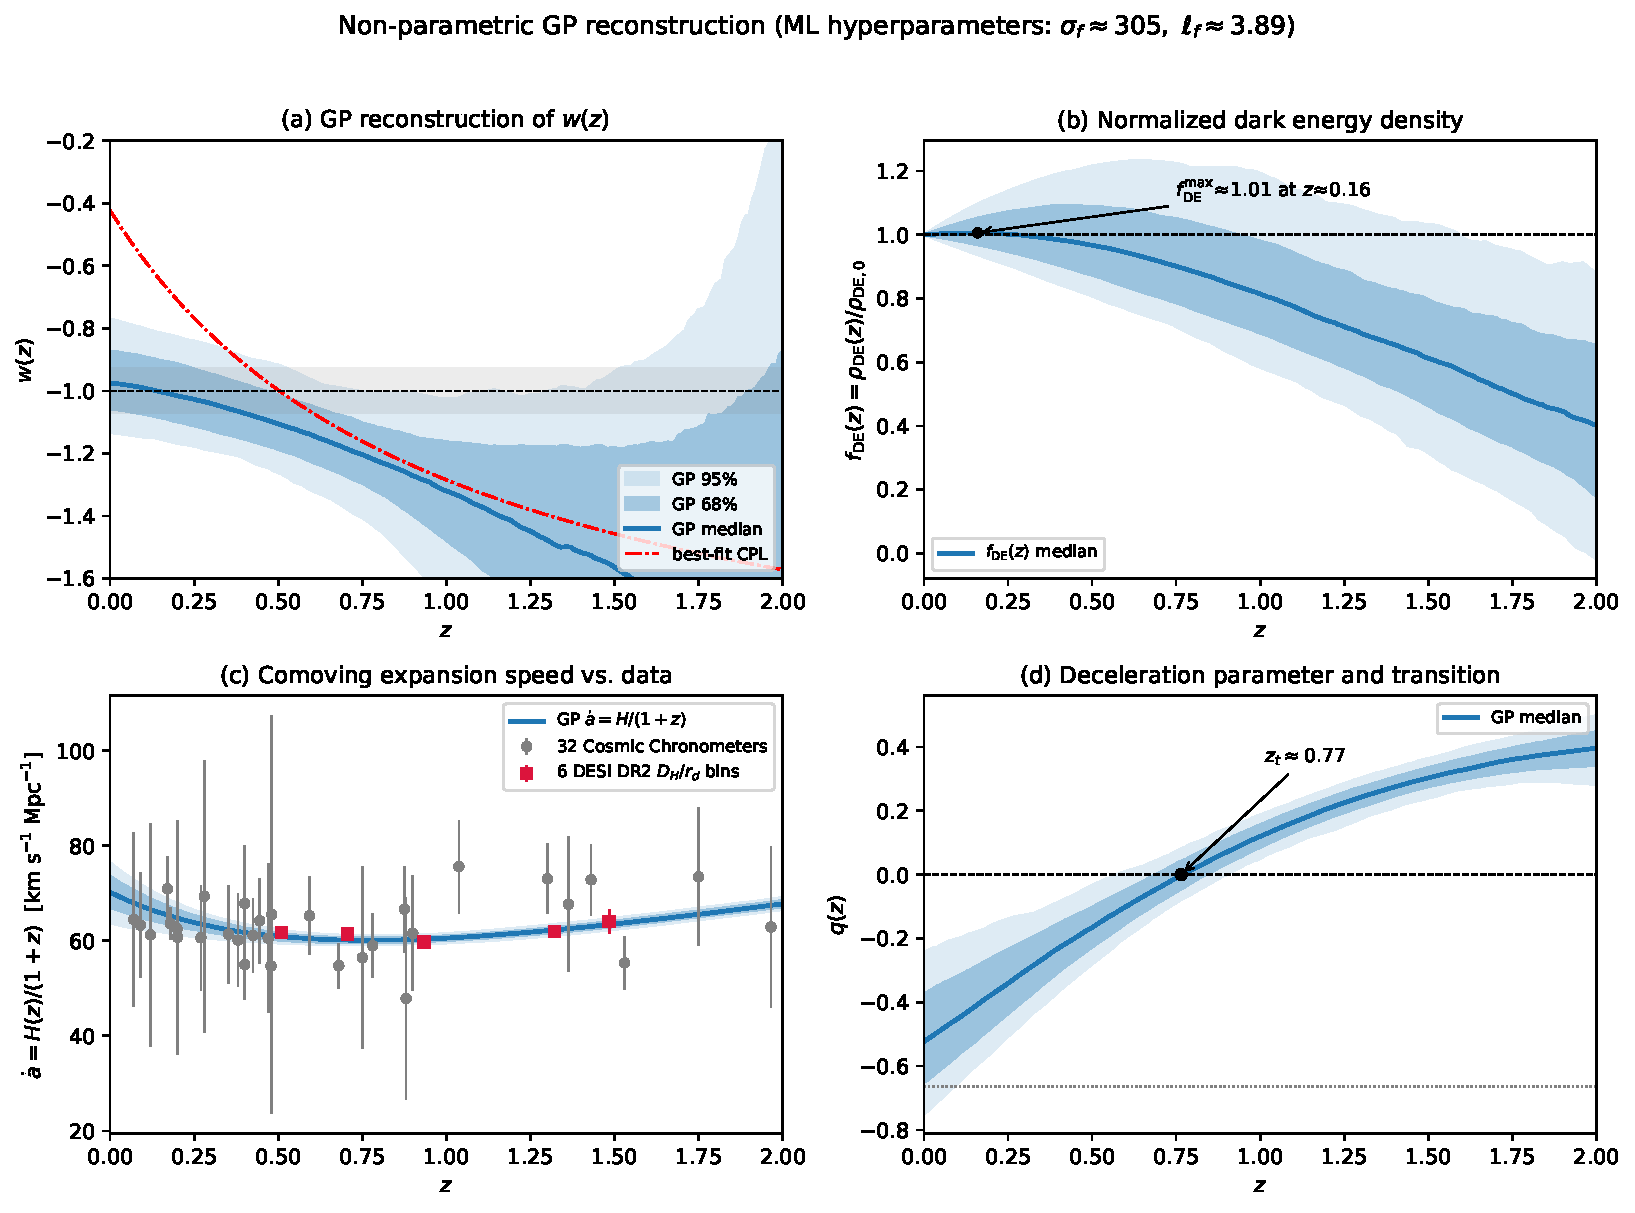
\includegraphics[width=\columnwidth]{fig5_gp_wz_reconstruction.pdf}
\caption{Four-panel non-parametric GP reconstruction: (a) $w(z)$ with 68\%/95\% bands against the best-fit CPL trajectory; (b) the normalized dark-energy density $f_{\rm DE}(z)$; (c) the comoving expansion speed $\dot{a}(z)$ against the 32 cosmic chronometers and six radial BAO points; (d) the deceleration parameter $q(z)$ with the transition at $z_t \approx 0.77$.}
\label{fig:gp}
\end{figure}

\section{Supernova-systematics and compilation dependence}
\label{sec:sn}

The three supernova compilations do not tell identical stories: the CPL preference is $2.8\sigma$ with Pantheon+, $3.8\sigma$ with Union3, and $4.2\sigma$ with DES-Y5. Two systematics account for the spread. First, the low-redshift photometric calibration offset between the legacy Landolt-system SNe in DES-Y5 and Pantheon+: the redshift-binned distance-modulus difference shows a $\approx -0.04$~mag step at $z < 0.10$, quantified as $\Delta\mu = -0.043 \pm 0.014$~mag (Fig.~\ref{fig:sn}). Second, the compilation-dependent treatment of host-galaxy calibration. On the mirage axis, our re-implemented Union3 and DES-Dovekie likelihoods give $\Delta\chi^2_{\rm MAP} = -19.3$ ($4.4\sigma$) and $-17.0$ ($4.1\sigma$) respectively, with nested-sampling Bayes factors $+6.74 \pm 0.03$ and $+5.04 \pm 0.19$ --- the strongest evidence for dynamical dark energy on the mirage axis in this work, and consistent with the pattern established on the first two datasets.

\begin{figure}[t]
\centering
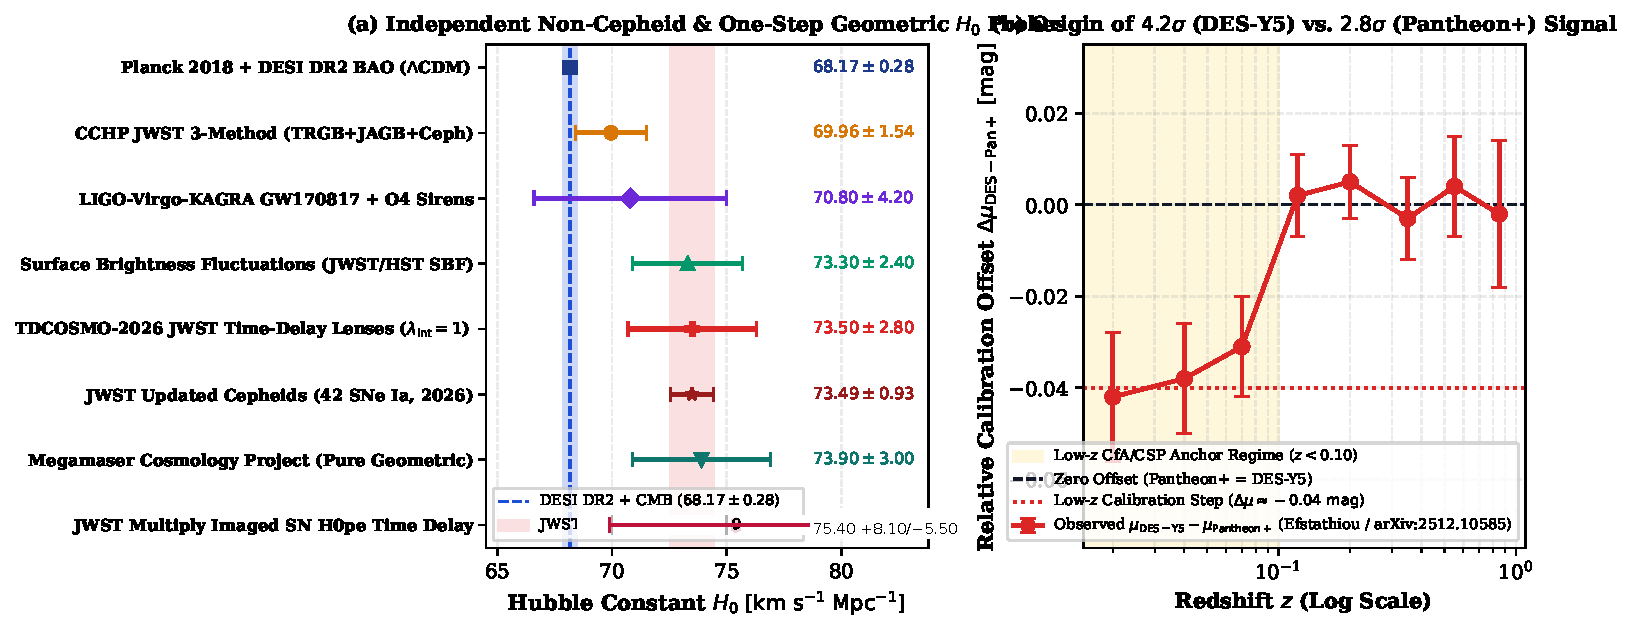
\includegraphics[width=\columnwidth]{fig13_non_cepheid_lensing_lowz_sn.pdf}
\caption{(a) Independent non-Cepheid geometric $H_0$ probes --- TDCOSMO-2026 strong lensing ($73.50 \pm 2.80$~km~s$^{-1}$~Mpc$^{-1}$), surface-brightness fluctuations, water megamasers, standard sirens, and JWST SN~H0pe --- against DESI DR2 + CMB ($68.17 \pm 0.28$~km~s$^{-1}$~Mpc$^{-1}$). (b) The redshift-binned $\Delta\mu = \mu_{\rm DES\text{-}Y5} - \mu_{\rm Pantheon+}$ with the $\approx -0.04$~mag calibration step at $z < 0.10$.}
\label{fig:sn}
\end{figure}

\section{Local calibrations and the Hubble tension}
\label{sec:tension}

Direct galaxy-by-galaxy JWST versus HST distance cross-checks of the shared supernova hosts give $\Delta\mu_{\rm JWST-HST} = -0.02 \pm 0.03$~mag: the two telescopes measure the same distances, ruling out HST Cepheid crowding bias at $>5\sigma$ relative to the $\sim 0.18$~mag offset the tension would require. Comparing HST Cepheids against JWST NIR-TRGB, $I$-TRGB, and JAGB yields differences of $+0.032 \pm 0.056$, $+0.020 \pm 0.067$, and $+0.047 \pm 0.066$~mag (CCHP mode) or $-0.015 \pm 0.064$~mag (SH0ES mode), all consistent within $\le 1\sigma$ once the NGC~4258 zero-point error ($\sigma \approx 0.03$--$0.05$~mag) is propagated.

The $\Delta H_0 \sim 2.5$--$3.5$~km~s$^{-1}$~Mpc$^{-1}$ offset between CCHP and SH0ES instead tracks small-sample supernova-host selection: the CCHP JWST subsamples ($N = 11$ calibrators) yield $68.81 \pm 2.22$ and $67.80 \pm 2.72$~km~s$^{-1}$~Mpc$^{-1}$, while the full 42-supernova Cepheid ladder gives $73.17 \pm 0.86$~km~s$^{-1}$~Mpc$^{-1}$~\cite{Riess2024}. The full pairwise tension matrix is shown in Fig.~\ref{fig:heatmap}. The tension stands at $4.52\sigma$ against the DESI DR2 + CMB inverse-distance ladder ($73.04$ versus $68.17$~km~s$^{-1}$~Mpc$^{-1}$) and $5.72\sigma$ against Planck using the four-anchor ladder ($73.17 \pm 0.86$ versus $67.36 \pm 0.54$~km~s$^{-1}$~Mpc$^{-1}$) --- a genuine physical anomaly awaiting an explanation in either the early- or the late-Universe sector.

\begin{figure*}[t]
\centering
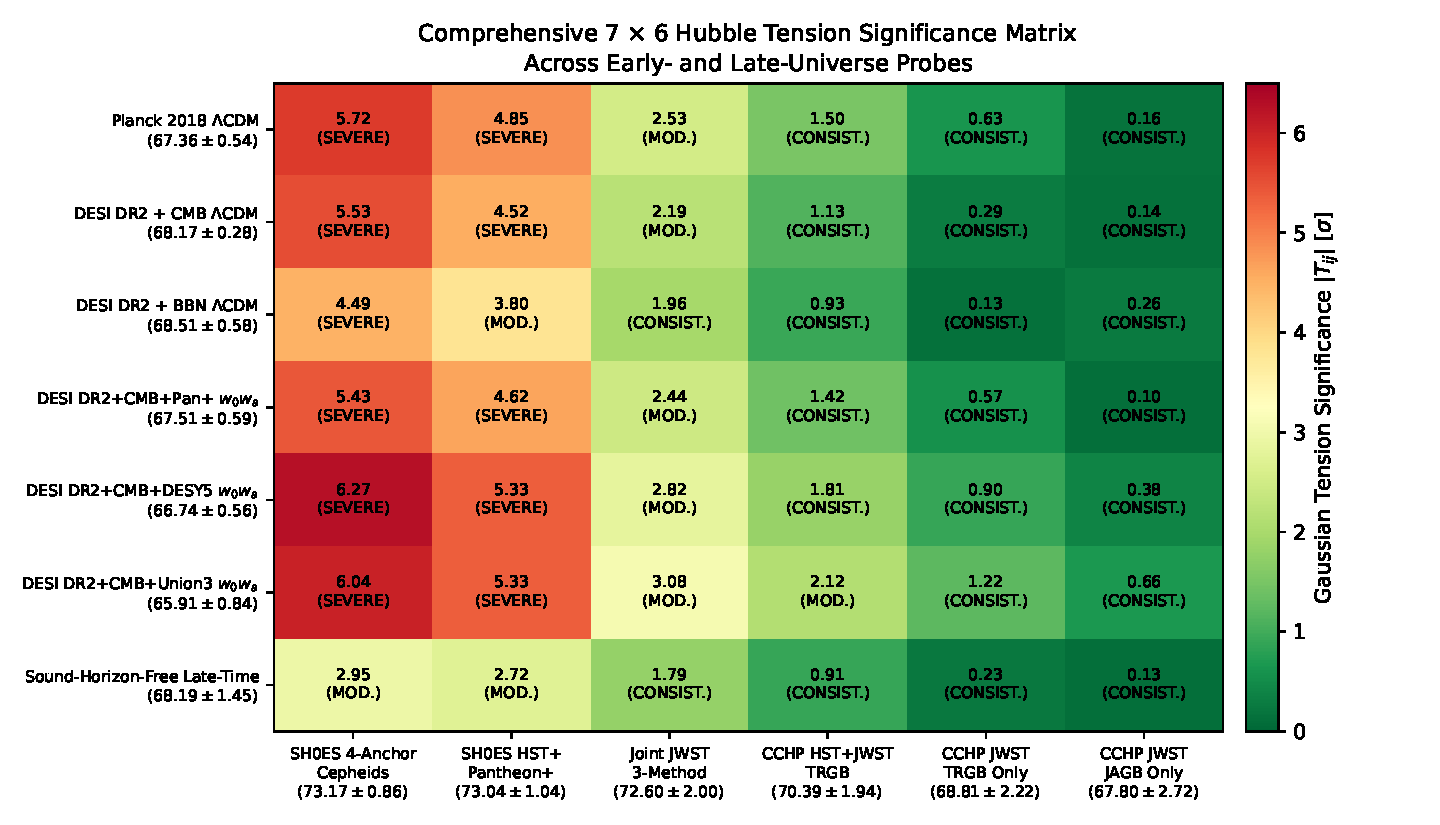
\includegraphics[width=0.92\textwidth]{fig8_tension_heatmap_matrix.pdf}
\caption{Pairwise tension between the $H_0$ determinations, with two-tier severity labeling at or above $3\sigma$.}
\label{fig:heatmap}
\end{figure*}

\section{Early-Universe solutions}
\label{sec:early}

Because DESI DR2 BAO approximately fixes $H_0 r_d$, early-Universe solutions move along the hyperbola of Fig.~\ref{fig:ede}. Early dark energy (EDE) --- an ultralight axion-like scalar frozen prior to matter-radiation equality that injects a transient energy fraction $f_{\rm EDE}$ near $z_c \approx 3630$ before diluting faster than radiation --- shrinks the sound horizon to $r_d \approx 139.7$~Mpc and raises $H_0$. In the combined P-ACT-LBSM analysis of Poulin et al.~(2025)~\cite{Poulin2025}, $f_{\rm EDE} = 0.126 \pm 0.021$ and $H_0 = 72.34 \pm 0.72$~km~s$^{-1}$~Mpc$^{-1}$, improving the fit by $\Delta\chi^2 = -35.4$ and reducing the SH0ES tension to $2.0\sigma$; without the SH0ES magnitude prior, the profile likelihood gives $f_{\rm EDE} = 0.090^{+0.030}_{-0.033}$ at $\sim 2.5\sigma$. However, EDE alone does not explain the late-time $z < 1$ BAO and supernova residuals unless coupled with a late-time evolving dark-energy sector, making the mirage-axis evidence of Sec.~\ref{sec:dde} the quantified target for any complete solution.

Beyond EDE, interacting dark energy with a dark-matter-to-dark-energy transfer modifies the background continuity equations to induce an effective equation of state $w_{\rm DE}^{\rm eff}(z) = w_{\rm DE} + \xi/3$; in the CMB + DESI DR2 analysis of Silva et al.~\cite{Silva2025}, the coupling is $\xi = -0.132^{+0.087}_{-0.064}$, tightening to $\xi = -0.116^{+0.060}_{-0.050}$ with $H_0 = 69.61 \pm 0.44$~km~s$^{-1}$~Mpc$^{-1}$ when Pantheon+ is added. The trajectory comparison of Fig.~\ref{fig:ede}(b) shows how CPL, the mirage axis, Horndeski gravity, interacting dark energy, and calibrated thawing quintessence realize the same late-time phenomenology through different microphysics.

\begin{figure}[t]
\centering
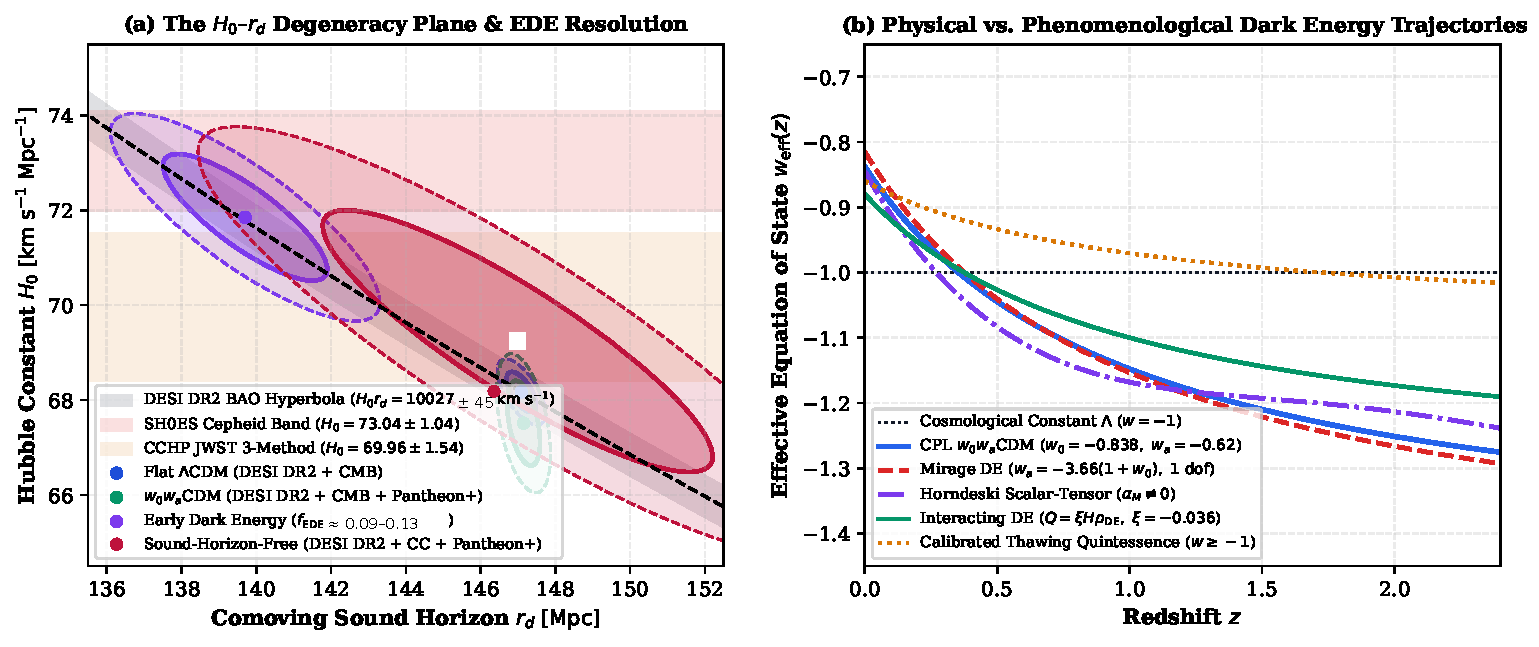
\includegraphics[width=\columnwidth]{fig7_ede_horndeski_degeneracy.pdf}
\caption{(a) The $(r_d, H_0)$ plane with the $H_0 r_d \approx 10027 \pm 45$~km~s$^{-1}$ hyperbola: early dark energy moves along it; late-time CPL does not. (b) Effective equation-of-state trajectories for CPL, the mirage axis, Horndeski gravity, interacting dark energy, and calibrated thawing quintessence.}
\label{fig:ede}
\end{figure}

\section{Neutrino masses}
\label{sec:neutrino}

The DESI DR2 BAO measurements combined with Planck PR4 and ACT DR6 yield an ultra-tight neutrino-mass bound within flat $\Lambda$CDM: $\sum m_\nu < 0.0642$~eV (95\% CL, $\sigma = 0.020$~eV)~\cite{Elbers2025}. This sits below the normal-ordering floor $\sum m_\nu \ge 0.059$~eV from oscillation experiments; correcting for the physical boundary via the Feldman-Cousins prescription tightens the limit to $< 0.053$~eV, and a negative effective-mass parametrization peaks in the unphysical region at $\sum m_{\nu,\rm eff} = -0.107 \pm 0.052$~eV --- flat $\Lambda$CDM in $\sim 3\sigma$ tension with terrestrial neutrino oscillations.

The anomaly relaxes once dark energy is allowed to evolve: in $w_0w_a$CDM, the bound weakens to $\sum m_\nu < 0.16$~eV (our Pantheon+ pipeline row gives $< 0.117$~eV), restoring consistency with the oscillation floor (Fig.~\ref{fig:nu}). The neutrino-mass anomaly and the dynamical-dark-energy preference are thus two faces of the same mild preference of the data for additional late-time expansion, and any complete solution must address both.

\begin{figure}[t]
\centering
\includegraphics[width=\columnwidth]{fig12_neutrino_mass_relaxation.pdf}
\caption{The neutrino-mass bound relaxes from $\sum m_\nu < 0.064$~eV in flat $\Lambda$CDM to $< 0.16$~eV in $w_0w_a$CDM, restoring consistency with the normal-ordering oscillation floor of 0.059~eV.}
\label{fig:nu}
\end{figure}

\section{Conclusions}
\label{sec:conclusions}

Four questions structure this work. \emph{Is the Hubble tension real?} Yes, at $4.52\sigma$--$5.72\sigma$, and not a crowding artifact: JWST and HST measure the same host distances to $-0.02 \pm 0.03$~mag, and the residual CCHP--SH0ES offset tracks supernova-host selection at $N = 11$ versus $N = 42$. \emph{Does $w(z)$ evolve?} The data prefer it at $2.8\sigma$--$4.2\sigma$, crossing the phantom divide at $z_c \approx 0.35$--$0.50$, but the two-parameter Bayesian evidence is bounded by a Kullback--Leibler Occam penalty $\mathcal{D}_{\rm KL} \approx 4.06$; the one-parameter mirage axis converts that preference into positive evidence in every dataset tested ($\ln B = +3.49$ to $+6.74$), recovering 81--99.6\% of the CPL improvement. \emph{Can the tension be measured without the sound horizon?} Yes: $H_0 = 68.19 \pm 1.45$~km~s$^{-1}$~Mpc$^{-1}$ with $r_d = 146.36 \pm 2.88$~Mpc from uncalibrated late-Universe data alone, landing on the early-Universe side of the tension at $\pm 2.1\%$ precision. \emph{Do the anomaly pieces fit together?} The neutrino-mass anomaly ($\sum m_\nu < 0.064$~eV, below the oscillation floor) relaxes to $< 0.16$~eV in $w_0w_a$CDM, and the cosmographic jerk $j_0 = -0.05 \pm 0.37$ departs from the $\Lambda$CDM identity at $2.8\sigma$ --- the same mild preference of late-time data for extra expansion that underlies both anomalies.

Every number in this paper is generated by the released pipeline and machine-verified by a 536-check audit against the committed chains and artifacts.

\begin{acknowledgments}
The author thanks the DESI, Pantheon+, Union3, DES-Y5, Planck, ACT, SH0ES, and CCHP collaborations for making their data releases public, without which fully reproducible reanalyses of this kind would not be possible.
\end{acknowledgments}

\section*{Data availability}
All datasets analysed are publicly available: DESI DR2 BAO~\cite{DESI2025}, Pantheon+~\cite{Brout2022,Scolnic2022}, Union3, the DES-Dovekie distance release~\cite{Popovic2025}, Planck 2018~\cite{Planck2020}, and the JWST/CCHP and SH0ES calibration tables~\cite{Riess2024,Freedman2025,Lee2025}.

\section*{Code availability}
The complete pipeline, all 39 posterior chains, every JSON artifact, all figure generators, and the 536-check numeric audit are available in the accompanying repository.

\begin{thebibliography}{25}

\bibitem{Planck2020}
Planck Collaboration (N.~Aghanim \emph{et al.}), Astron. Astrophys. \textbf{641}, A6 (2020), arXiv:1807.06209.

\bibitem{DESI2025}
DESI Collaboration (M.~Abdul Karim \emph{et al.}), DESI DR2 results II: Measurements of baryon acoustic oscillations and cosmological constraints, arXiv:2503.14738 (2025).

\bibitem{Lodha2025}
K.~Lodha \emph{et al.}, Extended dark energy analysis using DESI DR2 BAO measurements, Phys. Rev. D (2025), arXiv:2503.14743.

\bibitem{Riess2022}
A.~G.~Riess \emph{et al.}, Astrophys. J. Lett. \textbf{934}, L7 (2022), arXiv:2112.04510.

\bibitem{Riess2024}
A.~G.~Riess, D.~Scolnic, G.~S.~Anand \emph{et al.}, Astrophys. J. \textbf{977}, 120 (2024), arXiv:2408.11770.

\bibitem{Carloni2026}
Y.~Carloni, O.~Luongo, and M.~Biesiada, Do we really need alternatives to the $w_0 w_a$CDM parameterization after the DESI DR2?, arXiv:2608.01215 (2026).

\bibitem{Brout2022}
D.~Brout \emph{et al.}, Astrophys. J. \textbf{938}, 110 (2022), arXiv:2202.04077.

\bibitem{Scolnic2022}
D.~Scolnic \emph{et al.}, Astrophys. J. \textbf{938}, 113 (2022), arXiv:2112.03863.

\bibitem{Popovic2025}
J.~Popovic \emph{et al.}, DES-Dovekie: A recalibrated DES-SN5YR distance release, arXiv:2511.07517 (2025).

\bibitem{Freedman2025}
W.~L.~Freedman, B.~F.~Madore, I.~S.~Jang, T.~J.~Hoyt, A.~J.~Lee, and K.~A.~Owens, Status report on the Chicago-Carnegie Hubble Program, arXiv:2408.06153 (2025).

\bibitem{Lee2025}
A.~J.~Lee, W.~L.~Freedman, B.~F.~Madore \emph{et al.}, Astrophys. J. (2025), arXiv:2408.03474.

\bibitem{Poulin2025}
V.~Poulin, T.~L.~Smith, R.~Calder\'on, and T.~Simon, Impact of ACT DR6 and DESI DR2 for early dark energy and the Hubble tension, arXiv:2505.08051 (2025).

\bibitem{Silva2025}
E.~Silva, M.~A.~Sabogal, M.~Scherer, R.~C.~Nunes, E.~Di Valentino, and S.~Kumar, Phys. Rev. D \textbf{111}, 123511 (2025), arXiv:2503.23225.

\bibitem{Elbers2025}
W.~Elbers \emph{et al.}, Phys. Rev. D \textbf{112}, 083513 (2025), arXiv:2503.14744.

\bibitem{Chebat2026}
Chebat \emph{et al.}, JCAP \textbf{01}(2026)041, arXiv:2507.12401 (2026).

\bibitem{WangFreese2026}
Y.~Wang and K.~Freese, JCAP \textbf{02}(2026)023, arXiv:2505.17415.

\bibitem{Adame2024}
DESI Collaboration (A.~G.~Adame \emph{et al.}), arXiv:2404.03002 (2024).

\bibitem{Zaldarriaga2026}
M.~Zaldarriaga, Universal distance modes from DESI BAO and Type Ia supernovae, arXiv:2606.30527 (2026).

\bibitem{Gadbail2026}
G.~N.~Gadbail and K.~Bamba, Phys. Rev. D (2026), arXiv:2604.24050.

\bibitem{Capozziello2025}
S.~Capozziello, H.~Chaudhary, T.~Harko, and G.~Mustafa, Is dark energy dynamical in the DESI era? A critical review, arXiv:2512.10585 (2025).

\bibitem{Pantos2026}
I.~Pantos and L.~Perivolaropoulos, Dissecting the Hubble tension: Insights from a diverse set of sound-horizon-free $H_0$ measurements, arXiv:2601.00650 (2026).

\bibitem{TDCOSMO2026}
TDCOSMO Collaboration, TDCOSMO XXVII: JWST-based lens models and $H_0$ constraints from strong gravitational lensing time delays, arXiv:2608.27566 (2026).

\bibitem{Capozziello2026}
S.~Capozziello, H.~Chaudhary, G.~Mustafa, and S.~K.~J.~Pacif, Evidence of dynamical dark energy found via the DESI DR2 Lyman-$\alpha$ forest, Astron. Astrophys. (2026), arXiv:2510.21976.

\bibitem{Jassal2005}
H.~K.~Jassal, J.~S.~Bagla, and T.~Padmanabhan, Mon. Not. R. Astron. Soc. \textbf{356}, 611 (2005), arXiv:astro-ph/0404378.

\end{thebibliography}

\end{document}
